\documentclass[svgnames,14pt]{beamer}
\usepackage[utf8]{inputenc}
\usepackage{caption}
\usepackage{graphicx}
\usepackage{xcolor}
\usepackage{wrapfig}
\usepackage{algorithm}
\usepackage{algpseudocode}
\title{The 3D Organization of Chromatin Explains Evolutionary Fragile Genomic Regions by \\ \vspace{12pt} \normalsize{Camille Berthelot, Matthieu Muffato, \\ Judith Abecassis and Hugues Roest Crollius} }
\author{Speaker: Ilia Minkin}
\institute{}
\algnotext{EndFor}
\algnotext{EndIf}
\algnotext{EndWhile}
\setbeamertemplate{footline}[frame number]
\setbeamertemplate{navigation symbols}{}
\setbeamertemplate{caption}[numbered]
\captionsetup[figure]{labelformat=empty}

\begin{document}

\date{24th April 2015}
\maketitle

\begin{frame}
\frametitle{Two types of genome alterations}

1. Small point mutations:

{\vspace{12pt} \Large \color{Blue}
ACTTG\\
A{\color{Red}G}T--\hspace{2.7pt}G
\vspace{12pt}}

\pause
2. Large rearrangements:
\begin{itemize}
\item Inversions
\item Transpositions
\item Fusions
\item ...
\end{itemize}
\end{frame}

\begin{frame}
\frametitle{Genome Rearrangements}
\begin{figure}
	\centering
	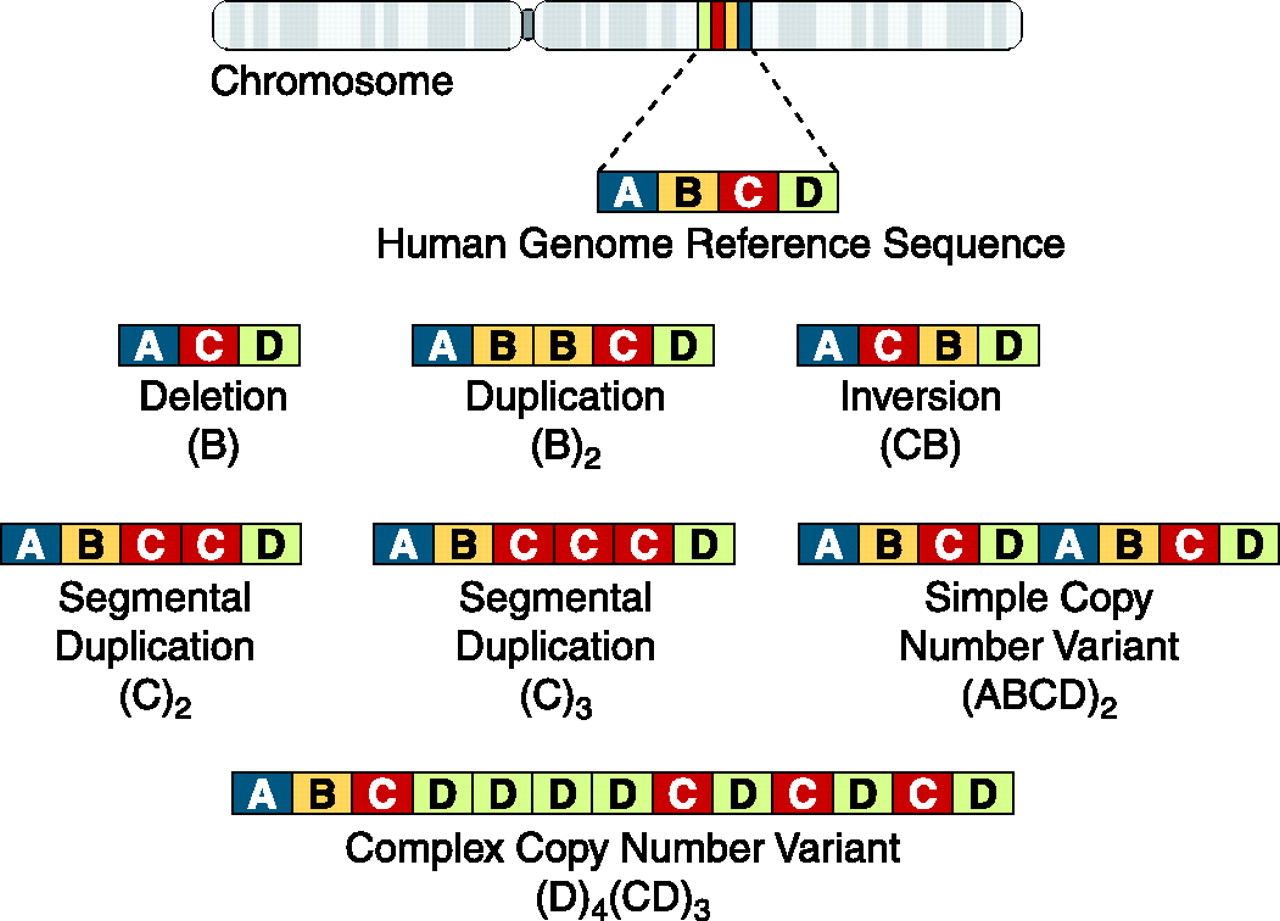
\includegraphics[scale = 0.20]{BasicRearr.jpg}
\caption{Source: \textit{Dierssen et al, 2009}}
\end{figure}
\end{frame}

\begin{frame}
\frametitle{Motivation}
Rearrangements:
\begin{itemize}
\item Are a major driving force in evolution
\item Play large role in diseases (e.g. cancer)
\end{itemize}
Known mechanisms:
\begin{itemize}
\item Non-homologous end joining
\item Non-allelic homologous recombination
\item Replication fork stalling
\item ...
\end{itemize}
\end{frame}

\begin{frame}
\frametitle{The Big Question}
Are rearrangements more likely to happen in one parts of a genome than the others?
\pause

\vspace{12pt}
Two hypotheses:
\begin{enumerate}
\item Rearrangements are distributed uniformly
\item Some regions are more likely to be disrupted
\end{enumerate}
\end{frame}

\begin{frame}
\frametitle{A Short Survey}
In 1984, Nadeau and Taylor presented first arguments in favor of random breakage

\pause
\vspace{12pt}
Pevzner and Tesler in 2003 showed evidence of fragile regions

\pause
\vspace{12pt}
Ma et al., 2006 argued for random model with higher resolution analysis of rearrangements 

\pause
\vspace{12pt}
Alekseyev and Pevzner, 2010 proposed that fragile regions may born and die

\pause
\vspace{12pt}
The story is to be continued...
\end{frame}

\begin{frame}
\frametitle{The Study}
Two questions:
\begin{itemize}
\item Do fragile regions exist?
\item If they do, what is cause of fragility?
\end{itemize}

\vspace{12pt}
A note: fragility is not "physical", it only means higher possibility of rearrangements
\end{frame}

\begin{frame}
\frametitle{Genomes Representations}
Genomes are sequences of gene markers that are unbreakable:
\begin{figure}
	\centering
	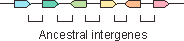
\includegraphics[scale = 2.20]{Intergenes.pdf}
\end{figure}

\pause
\vspace{12pt}
Here red dashes are breakpoints:
\begin{figure}
	\centering
	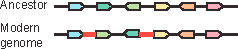
\includegraphics[scale = 2.20]{Breakpoint.pdf}
\end{figure}
\end{frame}

\begin{frame}
\frametitle{Methodology}
Suppose that we have an ancestral genome and its successors
\begin{figure}
	\centering
	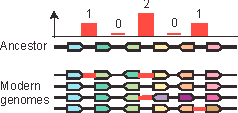
\includegraphics[scale = 2.20]{Ancestor.pdf}
\end{figure}

How does ancestral intergene length affects its breakage rate?
\end{frame}

\begin{frame}
\frametitle{Methodology}
Null hypothesis: breakpoint density is uniform

\vspace{12pt}
As intergene length $\Uparrow$, \# of breakpoints $\Uparrow$ as well

\vspace{12pt}
It yields Poisson distribution of breakage rate
\end{frame}

\begin{frame}
\frametitle{Methodology}
Boreoeutheria: the last common ancestor of primates, rodents, and laurasiatherians

\vspace{12pt}
Stages of the study:
\begin{itemize}
\item Reconstruct gene order of Boreoeutheria
\item Annotate ancestral intergenes
\item Identify breakpoints w.r.t. human, mouse, dog, cow and horse
\item Do Poisson regression of "breakage rate" 
\end{itemize}

\vspace{12pt}
Expect linear law if the null hypothesis is true
\end{frame}

\begin{frame}
\frametitle{Intergene Annotation}
\begin{figure}
	\centering
	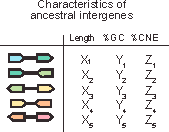
\includegraphics[scale = 2.20]{Annotation.pdf}
\end{figure}
\end{frame}


\begin{frame}
\frametitle{How to Explain the Equation?}
$$r = 2.4 10^{-3} \times L ^ {0.38}$$

93\% of variation in breakpoint occurrence is explained by intergene length

\vspace{12pt}
Maybe GC content is the real cause?
\end{frame}

\begin{frame}
\frametitle{Is GC Content The Explanation?}
No.
\vspace{12pt}

\pause
Added GC content in regression -- non-significant coefficient
\end{frame}

\begin{frame}
\frametitle{Are CNEs The Explanation?}
CNEs -- conservative non-coding elements.

Located in the intergenes, may affect rearrangement rate.
Do they?
\vspace{12pt}

\pause
No.
\vspace{12pt}

\pause
Added CNE rate in regression -- improved explanation rate only by 3\%
\end{frame}

\begin{frame}
\frametitle{Inversions within Intergenes}
OK, maybe some breakpoints are more likely than the others.

\vspace{12pt}
We work with gene markers --- see only rearrangements disrupting their order.

\vspace{12pt}
What if there are many missing rearrangements within intergenes?

\vspace{12pt}
We can try to simulate rearrangements and see what happens
\end{frame}

\begin{frame}
\frametitle{Inversions within Intergenes}
Rearrangements have been shown to occur between regions in close 3D proximity in the nucleus

\vspace{12pt}
Contact probability is a good proxy for rearrangement probability

\vspace{12pt}
Simulate and sample breakpoint pairs, choose detectable ones

\vspace{12pt}
Even if we restrict to detectable breakpoints only, simulation confirms the random breakpoint hypothesis
\end{frame}

\begin{frame}
\frametitle{Open Chromatin is the Culprit}
Stick with the simulation -- restrict rearrangements to only \textbf{open chromatin} regions

\vspace{12pt}
Voilà -- simulation coincides with the model!

It implies that chromatin state and proximity of genes may explain fragility of some genomic regions
\end{frame}


\begin{frame}
\frametitle{Conclusion}
It seems that chromatin state and proximity of genes may explain fragility of some genomic regions
\end{frame}

\begin{frame}
\begin{center}
\hfill \huge \\
Thank you!
\end{center}
\end{frame}


\end{document}
